% ====================================================================== RELATED WORK
\section{Related Works}\label{sec2}

\subsection{Matrix factorization and the cold-start problem}
Matrix factorization (MF) is the workhorse of collaborative filtering~\cite{koren2009mf}. Each user $u$ and item $i$ are mapped to latent vectors $p_u, q_i \in \mathbb{R}^d$, and their affinity is modelled as $\hat r_{ui} = \mu + b_u + b_i + \langle p_u, q_i\rangle$. The weakness of MF is structural: a user who does not appear in the training data has no vector, which is the classic cold-start problem~\cite{schein2002coldstart}. In fashion this is the common case rather than the exception, because most shoppers buy only a handful of items.

\subsection{Ordinal regression}
Fit feedback is ordered (\emph{small} $<$ \emph{fit} $<$ \emph{large}). The cumulative-link model~\cite{mccullagh1980ordinal} uses one latent score $t$ and ordered thresholds $\theta_1 < \theta_2$, $P(y \le k) = \sigma(\theta_k - t)$. A large $t$ means that the article is large for the wearer and a small $t$ means that it is tight. The formulation needs fewer parameters than a three-way classifier and respects the ordering of the labels.

\subsection{Size and fit recommendation}
Sembium et al.~\cite{sembium2017size} introduced latent ``true sizes'' for customers and products, learned from small/fit/large feedback. Misra et al.~\cite{misra2018fit} released the ModCloth and RentTheRunway datasets used in this work and proposed K-LF-ML, which combines $K$-dimensional latent factors, ordinal regression and metric learning to handle the subjectivity of fit feedback; it reached an AUC of 0.657 on ModCloth and 0.719 on RentTheRunway. Guigourès et al.~\cite{guigoures2018bayes} cast the problem as a hierarchical Bayesian model.

Sheikh et al.~\cite{sheikh2019sfnet} proposed SFNet, a deep content-collaborative network that combines user and item embeddings with customer and article attributes, reaching 0.689 and 0.749 AUC on the same two datasets. An important observation in that work is that removing the user ID barely changes the result, because most customers have a single transaction. This is direct evidence that collaborative embeddings are hard to learn on sparse fashion data and that another source of user information is needed.

Other directions include transformer models over purchase histories~\cite{eshel2021presize}, production systems that flag problematic articles from weak labels and expert priors~\cite{nestler2021sizeflags}, and the use of review text: Baier~\cite{baier2019reviews} predicted fit from reviews with a micro-F1 above 0.82, and Chatterjee et al.~\cite{chatterjee2022reviews} added review embeddings to a size recommender. Table~\ref{tab:related} summarises the works evaluated on the two datasets used here.

\begin{table}[h]
\caption{Representative studies on ModCloth (MC) and RentTheRunway (RTR)}\label{tab:related}
\begin{tabular*}{\textwidth}{@{\extracolsep\fill}p{2.1cm}p{3.6cm}p{2.0cm}p{3.6cm}}
\toprule
Study & Method & Result & Limitation \\
\midrule
Misra et al.~\cite{misra2018fit} & Latent factors + ordinal regression + metric learning (K-LF-ML) & AUC MC 0.657, RTR 0.719 & Body measurements not used directly; cold-start unresolved \\
Sheikh et al.~\cite{sheikh2019sfnet} & SFNet: deep network over embeddings and attributes & AUC MC 0.689, RTR 0.749 & Hard to interpret; user embeddings contribute almost nothing \\
Baier~\cite{baier2019reviews} & Fit prediction from review text (TF-IDF, ULMFiT, BERT) & Micro-F1 0.827 / 0.842 & Reviews exist only after purchase \\
Chatterjee et al.~\cite{chatterjee2022reviews} & Customer and product features + review embeddings & Macro-F1 gain over SFNet & ModCloth used only to train the language model \\
\botrule
\end{tabular*}
\end{table}

\subsection{Research gap}
Previous work has shown, separately, the value of latent collaborative factors, explicit customer and product attributes, and review text. What is still missing is a simple and interpretable MF model in which \emph{the collaborative latent factors are integrated directly with self-reported anthropometric information}, evaluated systematically by how much history a user has (none, one, a few, or many purchases). ModCloth and RentTheRunway are well suited to close this gap, because they contain both kinds of information: collaborative signals (\texttt{user\_id}, \texttt{item\_id}, \texttt{size}, \texttt{fit}) and body information (height, weight, bust, waist, hips, body type). To test the gap empirically we compare at least three configurations, MF alone, MF with body measurements, and MF with body measurements and product features, on new users and on users with sparse histories. Review text is only available after purchase, so it is not used as an input and is left for future work.

% ====================================================================== DATA
\section{Data}\label{sec3}

\subsection{Datasets}
We use the Clothing Fit Dataset of Misra et al.~\cite{misra2018fit}. \emph{ModCloth} is a women's clothing retailer and \emph{RentTheRunway} (RTR) is a platform for renting formal wear. Each record is one transaction with the customer, the article, the chosen size, the fit feedback and the body measurements reported by the customer. Table~\ref{tab:data} summarises both datasets after cleaning.

\begin{table}[h]
\caption{Dataset statistics after cleaning}\label{tab:data}
\begin{tabular*}{\textwidth}{@{\extracolsep\fill}lrr}
\toprule
 & ModCloth & RentTheRunway \\
\midrule
Transactions & 82,790 & 192,544 \\
Users & 47,958 & 105,571 \\
Items & 1,378 & 5,850 \\
Item--size pairs & 5,005 & 30,815 \\
Categories & 7 & 68 \\
Users with a single transaction & 66.5\% & 68.0\% \\
Small / fit / large (\%) & 15.7 / 68.6 / 15.8 & 13.4 / 73.8 / 12.8 \\
\botrule
\end{tabular*}
\end{table}

The two datasets expose different measurements. RTR provides height, weight, age, bra size (e.g.\ \texttt{34b}), body type (seven classes) and the rental occasion. ModCloth provides height, bra band, cup, bust, waist, hips and shoe size. This lets us check whether the model behaves consistently across two different measurement schemas.

\subsection{Exploratory analysis}
Figure~\ref{fig:data} highlights two properties. First, the labels are dominated by \emph{fit} (about 70\%), so a model that always predicts \emph{fit} already reaches about 70\% accuracy; accuracy is therefore misleading and we report macro AUC and macro-F1. Second, missingness varies widely: height is almost always present (under 2\% missing), whereas on ModCloth waist and bust are missing in more than 85\% of rows and hips in about 32\%, and on RTR weight is missing in about 16\%. The model must therefore handle missing values without discarding records. Sizes in both datasets have a median of about 12 and concentrate on sizes 4, 8 and 12.

\begin{figure}[h]
\centering
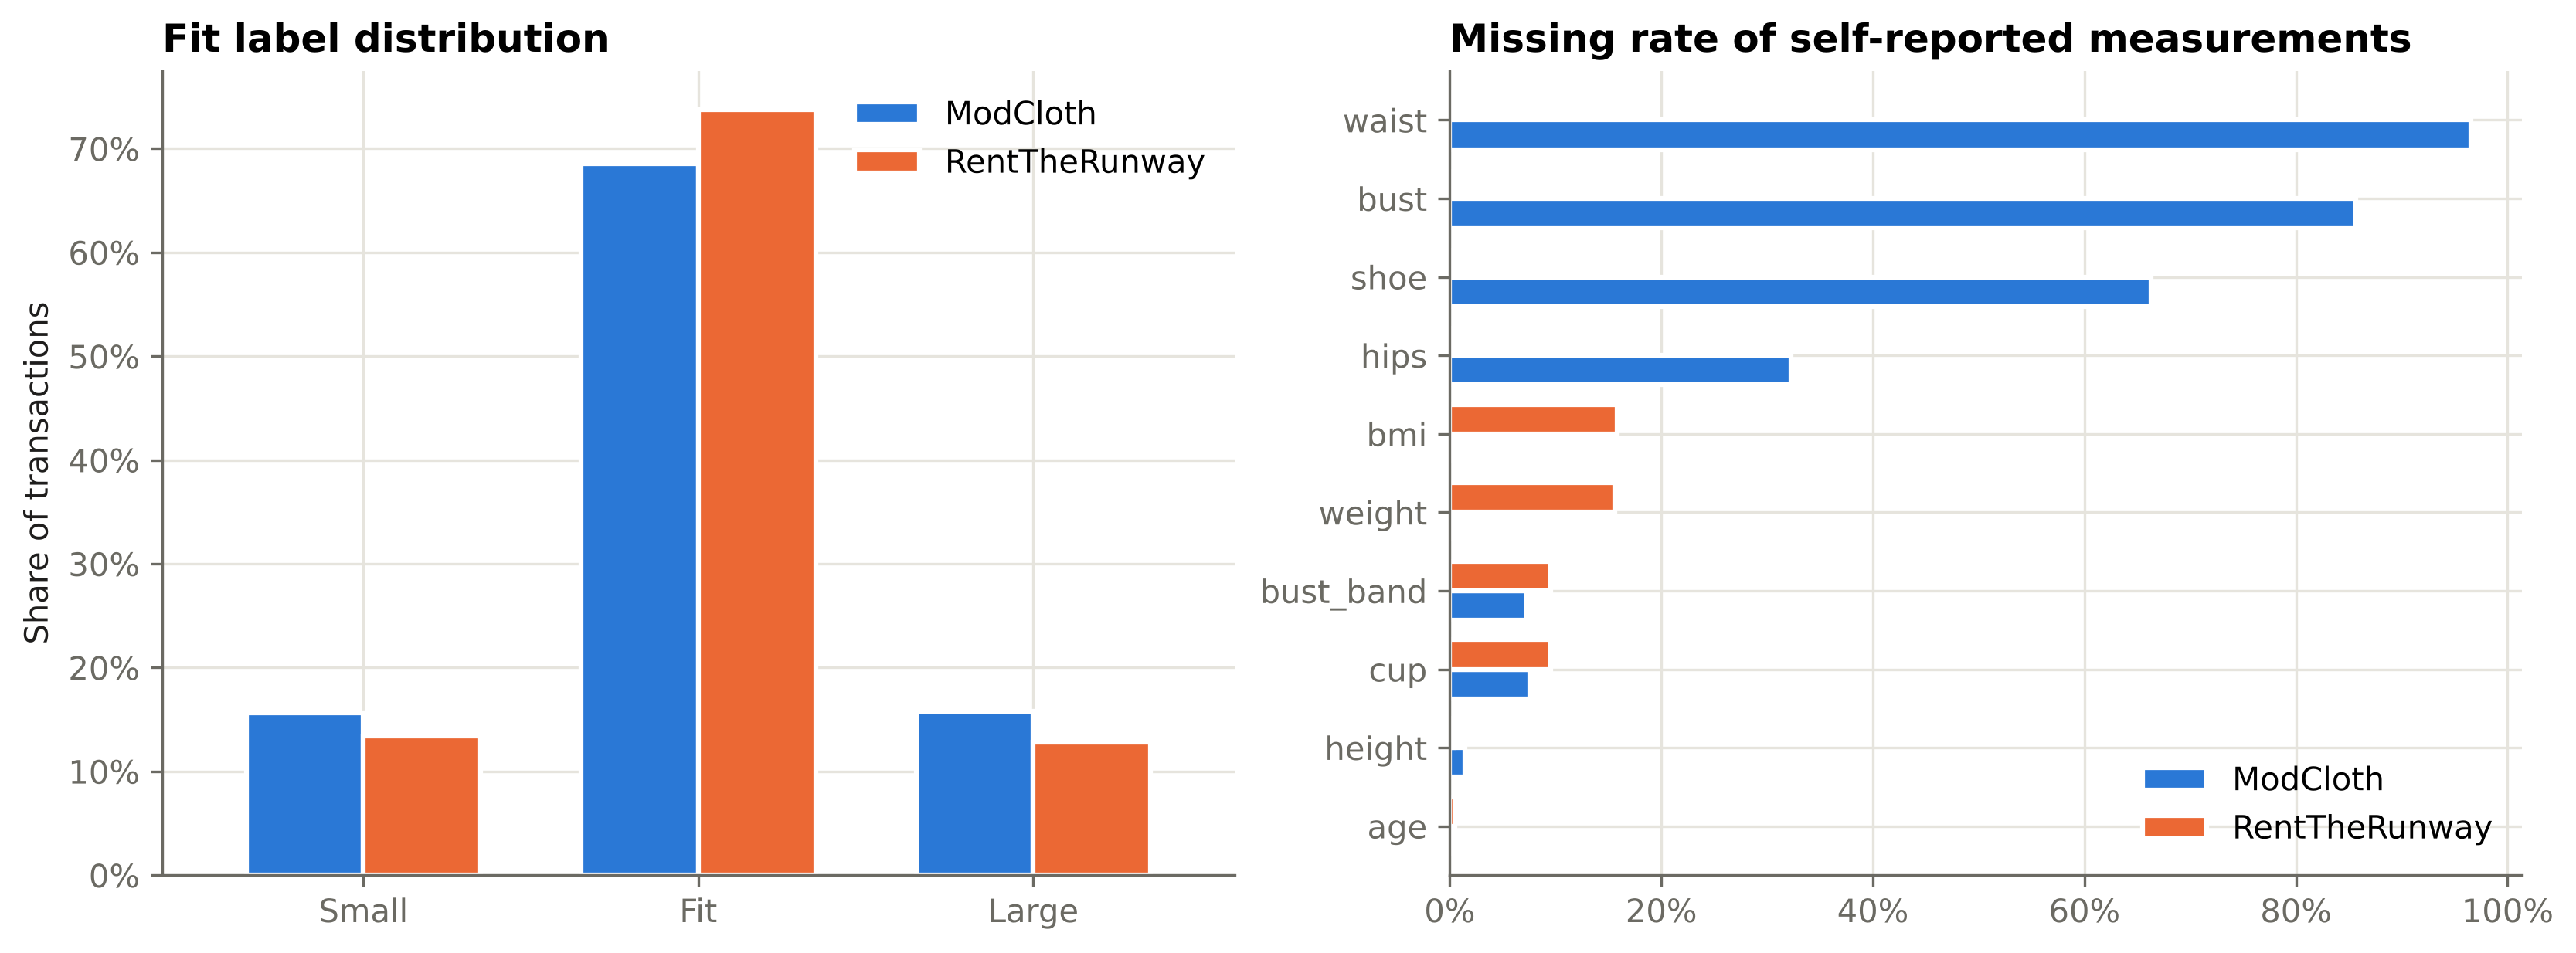
\includegraphics[width=0.9\textwidth]{fig1_data_overview.png}
\caption{Distribution of fit labels (left) and share of missing values per body measurement (right)}\label{fig:data}
\end{figure}

\subsection{Pre-processing}
\begin{itemize}
\item \textbf{Units.} Heights are converted to inches (accepting \texttt{5'6"} and \texttt{168cm}) and weights to pounds. Bra size is split into band and cup, and cups are encoded ordinally ($a<b<c<d<dd/e<\dots$). BMI is derived from height and weight, and implausible values are treated as missing.
\item \textbf{Encoding.} Measurements are z-scored using training statistics only. Missing values are imputed with 0 (the mean). A missingness indicator is added for every column that is missing in at least 2\% of training rows. Body type is one-hot encoded.
\item \textbf{Leakage control.} Fields that only exist after purchase (\texttt{review\_text}, \texttt{review\_summary}, \texttt{rating}, \texttt{quality}, \texttt{length}) are excluded. Users and items unseen during training map to an UNKNOWN index.
\end{itemize}

% ====================================================================== METHOD
\section{Proposed Method}\label{sec4}

The system has two components. A \textbf{hybrid ordinal MF} model predicts $P(\text{small})$, $P(\text{fit})$ and $P(\text{large})$ for a (customer, article, size) triple. A monotone \textbf{size-selection model} estimates the customer's target size for the article and returns the closest available size. The first model is then used to assess the risk of a bad fit at the selected size and to explain the recommendation.

\subsection{Hybrid ordinal matrix factorization}
Let $x_u$ be the encoded body measurements of user $u$, $i$ the article and $s$ the size. The model is
\begin{align}
\mathbf{u} &= m_u\,p_u + E(x_u), \label{eq:user}\\
\mathbf{v} &= q_{(i,s)} + q_i + c_{\mathrm{cat}(i)} + c_{\mathrm{ctx}} + z_s\,w + \mathrm{gap}\,w_{\mathrm{gap}}, \label{eq:item}\\
t &= \langle \mathbf{u}, \mathbf{v}\rangle + m_u\,b_u + b_{(i,s)} + b_i + g(x_u) + \beta\,\mathrm{gap}, \label{eq:score}\\
P(y \le k) &= \sigma(\theta_k - t), \qquad k \in \{\text{small}, \text{fit}\}. \label{eq:ord}
\end{align}
Here $p_u \in \mathbb{R}^{16}$ and $b_u$ are the collaborative latent vector and bias of the user. $E(\cdot)$ is a two-layer MLP (64 hidden units) that projects the body measurements into the \emph{same latent space} as $p_u$; this is the core of the hybrid design, because body information does not sit beside the collaborative part but builds the user representation directly. $m_u \in \{0,1\}$ equals 1 for users seen in training and 0 for new users, in which case $\mathbf{u} = E(x_u)$ and the prediction relies entirely on the measurements. $q_{(i,s)}$, $q_i$, $b_{(i,s)}$ and $b_i$ are the latent vectors and biases of the item--size pair and of the item, which capture whether an article runs large or small. $c_{\mathrm{cat}}$ and $c_{\mathrm{ctx}}$ embed the category and the usage context (the rental occasion on RTR), and $z_s$ is the standardised size; these explicit \emph{product features} help the model generalise to rare items and sizes. Finally, $g(x_u)$ is a linear term whose weights show the direct effect of each measurement.

\paragraph{Size-gap feature.} A ridge regression estimates the customer's ``natural'' size per category from body measurements, $\hat s(x_u, \mathrm{cat})$. The feature
\begin{equation}
\mathrm{gap} = \frac{s - \hat s(x_u, \mathrm{cat})}{\sigma_{\mathrm{resid}}}
\end{equation}
tells the model whether the size under consideration is large or small relative to the body. It plays the role of the latent ``true size'' of~\cite{sembium2017size,misra2018fit}, but is computed from the measurements and is therefore available for new users.

\paragraph{ID dropout.} During training the identity of the user is hidden ($m_u = 0$) for 10\% of the transactions. This forces the body branch $E(x_u)$ to predict well on its own, so the model serves new users, and lets $p_u$ learn only the personal preferences that the measurements cannot explain, such as a liking for loose or tight fits.

\paragraph{Training.} The loss is the negative log-likelihood of~\eqref{eq:ord} plus L2 regularisation ($\lambda = 10^{-2}$) on the embeddings in each batch. We use Adam~\cite{kingma2015adam} with learning rate $3\cdot10^{-3}$, batch size 1024, latent dimension $d=16$, at most 30 epochs, and early stopping when validation AUC does not improve for 3 epochs.

\subsection{Size selection}
Fit data are \emph{observational}: customers choose sizes close to their bodies, so almost no petite customer ever tries a size 20. A fit model with a good AUC is therefore unreliable when comparing distant sizes for the same person, which is a selection bias. We thus separate size selection into a monotone and interpretable model. For user $u$ and article $i$ in category $c$,
\begin{align}
\mathrm{base}_u &= \frac{n_u\,\mathrm{base}^{\mathrm{hist}}_u + k\,\hat s_{\mathrm{body}}(x_u)}{n_u + k}, \qquad k = 2,\\
\mathrm{target}_{u,i} &= \mathrm{base}_u + \delta_c + o_i,
\end{align}
where $\hat s_{\mathrm{body}}$ is the size estimated from the measurements, $\mathrm{base}^{\mathrm{hist}}_u$ is the base size learned from the user's $n_u$ past transactions (adjusted by their labels, e.g.\ shifted up if the user reported \emph{small}), $\delta_c$ is a category offset, and $o_i$ is how much the article runs large or small, learned from \emph{fit} transactions and shrunk towards zero for rare items. The recommended size is the available size closest to the target. A new user ($n_u = 0$) is served entirely from measurements, and the weight of the history grows with the number of purchases.

The hybrid model then estimates $P(\text{small})$, $P(\text{fit})$ and $P(\text{large})$ at the selected size. When the risk leans clearly to one side, the system suggests the neighbouring size \emph{only if} that size is actually safer: lower risk in that direction and no higher total risk of a bad fit.

% ====================================================================== EXPERIMENTS
\section{Experimental Setup}\label{sec5}

\subsection{Compared models}
All models share the same data splits and, except the first two baselines, the same ordinal loss (Table~\ref{tab:models}).

\begin{table}[h]
\caption{Model configurations}\label{tab:models}
\begin{tabular*}{\textwidth}{@{\extracolsep\fill}lcccl}
\toprule
Model & Collab. & Body & Product & Note \\
\midrule
\texttt{majority} & & & & Always predicts \emph{fit} \\
\texttt{body\_lr} & & \checkmark & \checkmark & Logistic regression on body, size, category \\
\texttt{mf} & \checkmark & & & Plain ordinal MF \\
\texttt{mf\_body} & \checkmark & \checkmark & & MF + body measurements \\
\texttt{body\_product} & & \checkmark & \checkmark & No user latent factor \\
\textbf{\texttt{mf\_body\_product}} & \checkmark & \checkmark & \checkmark & \textbf{Proposed} \\
\texttt{\dots\_nodrop} & \checkmark & \checkmark & \checkmark & Proposed without ID dropout \\
\botrule
\end{tabular*}
\end{table}

\subsection{Protocols}
\begin{itemize}
\item \textbf{Cold-start (user split).} Users are split 80/10/10 into train, validation and test, so every test user is new. This protocol mirrors the target scenario.
\item \textbf{Warm (transaction split).} Transactions are split 80/10/10 at random, and test results are broken down by the number of training transactions of the user: 0, 1, 2--4 and 5+. This shows how the contribution of the collaborative part changes as history grows.
\end{itemize}
Each protocol is repeated ten times with seeds 1--10; each seed produces a different split, and within a seed all models share the same split and are trained only on its training part. Results are reported as mean $\pm$ standard deviation over the ten repetitions.

\paragraph{Split design and leakage checks.} The warm protocol follows the random transaction split used by~\cite{misra2018fit,sheikh2019sfnet}, so its numbers can be set beside theirs; the cold-start protocol is stricter, because no test user appears in training. To prevent information from the test set reaching the model, every fitted component is estimated on the training part of each split only: the z-score statistics and missingness indicators of the body encoder, the ID mappings, the size standardisation, the ridge size regressor behind the gap feature, and the item offsets of the size-selection model. The validation part is used only for early stopping and for tuning the macro-F1 class weights, and the test part is used once, for the final scores. Post-purchase fields (reviews, rating, quality, length) are dropped before splitting. The only information taken from the whole catalogue is the list of sizes each article is offered in, which a shop knows before any sale. Before the full runs, the whole pipeline was tested on a small subset with a quick one-seed run (\texttt{run\_quick.sh} and an automated smoke test).

\subsection{Metrics and statistical tests}
\textbf{Macro AUC} (one-vs-rest, averaged over the three classes) is the primary metric, as in~\cite{misra2018fit,sheikh2019sfnet}; it is threshold-free and insensitive to the dominance of \emph{fit}. For \textbf{macro-F1} and accuracy, class weights for \emph{small} and \emph{large} are tuned on validation to maximise macro-F1 and then applied to test, because a plain argmax almost always returns \emph{fit}. \textbf{Size recommendation} is evaluated on test transactions labelled \emph{fit}, i.e.\ sizes the customer actually found to fit: we report the share of recommendations that match that size exactly and the share within one size step. This is the metric closest to the goal of reducing size-related returns.

The proposed model is compared with every other model by a \textbf{paired t-test} over the ten seeds and a \textbf{paired bootstrap}~\cite{efron1993bootstrap} with 200 resamples of the test set, pooled over seeds to obtain 95\% confidence intervals and p-values. Differences with $p < 0.05$ are considered significant.

% ====================================================================== RESULTS
\section{Results and Discussion}\label{sec6}

\subsection{Cold-start}
Table~\ref{tab:cold} reports results on new users. The proposed model achieves the highest AUC on both datasets, tied only with its own no-dropout ablation.

\begin{table}[h]
\caption{Cold-start protocol (mean $\pm$ std over 10 seeds; the proposed model is in bold)}\label{tab:cold}
\begin{tabular*}{\textwidth}{@{\extracolsep\fill}lcccc}
\toprule
 & \multicolumn{2}{c}{ModCloth} & \multicolumn{2}{c}{RentTheRunway} \\
\cmidrule{2-3}\cmidrule{4-5}
Model & AUC & Macro-F1 & AUC & Macro-F1 \\
\midrule
\texttt{majority} & 0.500 & 0.271 & 0.500 & 0.283 \\
\texttt{body\_lr} & 0.585 $\pm$ 0.003 & 0.379 $\pm$ 0.005 & 0.620 $\pm$ 0.004 & 0.421 $\pm$ 0.007 \\
\texttt{mf} & 0.661 $\pm$ 0.006 & 0.450 $\pm$ 0.030 & 0.722 $\pm$ 0.003 & 0.502 $\pm$ 0.004 \\
\texttt{mf\_body} & 0.674 $\pm$ 0.006 & 0.478 $\pm$ 0.007 & 0.724 $\pm$ 0.004 & 0.531 $\pm$ 0.006 \\
\texttt{body\_product} & 0.678 $\pm$ 0.007 & 0.486 $\pm$ 0.011 & 0.729 $\pm$ 0.004 & 0.524 $\pm$ 0.007 \\
\textbf{\texttt{mf\_body\_product}} & \textbf{0.679 $\pm$ 0.007} & \textbf{0.486 $\pm$ 0.009} & \textbf{0.731 $\pm$ 0.004} & \textbf{0.535 $\pm$ 0.007} \\
\texttt{\dots\_nodrop} & 0.679 $\pm$ 0.007 & 0.487 $\pm$ 0.009 & 0.731 $\pm$ 0.003 & 0.535 $\pm$ 0.007 \\
\botrule
\end{tabular*}
\end{table}

Body measurements mitigate cold-start: adding them to MF (\texttt{mf} $\rightarrow$ \texttt{mf\_body}) raises AUC by 0.013 on ModCloth and 0.002 on RTR, and adding product features (\texttt{mf\_body} $\rightarrow$ \texttt{mf\_body\_product}) adds a further 0.005 and 0.007. A linear model is not enough: \texttt{body\_lr} reaches only 0.585 and 0.620, because fit depends on the \emph{interaction} between a body and a specific item--size, not on either alone. For completely new users the proposed model and \texttt{body\_product} are close, which is expected since the two share the same form when $m_u = 0$.

\subsection{Effect of user history}
Table~\ref{tab:hist} and Figure~\ref{fig:hist} break down the warm protocol by the amount of user history.

\begin{table}[h]
\caption{Warm-protocol AUC by number of training transactions of the user (mean over 10 seeds; the standard deviation of the proposed model ranges from 0.004 to 0.015 across buckets)}\label{tab:hist}
\begin{tabular*}{\textwidth}{@{\extracolsep\fill}lccccc|ccccc}
\toprule
 & \multicolumn{5}{c|}{ModCloth} & \multicolumn{5}{c}{RentTheRunway} \\
Model & 0 & 1 & 2--4 & 5+ & All & 0 & 1 & 2--4 & 5+ & All \\
\midrule
\texttt{mf} & .658 & .669 & .663 & .671 & .663 & .728 & .723 & .726 & .722 & .724 \\
\texttt{mf\_body} & .671 & .676 & .676 & .689 & .675 & .725 & .725 & .730 & .727 & .727 \\
\texttt{body\_product} & .675 & .674 & .672 & .685 & .675 & .734 & .729 & .732 & .721 & .730 \\
\textbf{Proposed} & \textbf{.677} & \textbf{.681} & \textbf{.686} & \textbf{.698} & \textbf{.682} & \textbf{.735} & \textbf{.733} & \textbf{.739} & \textbf{.735} & \textbf{.736} \\
\midrule
Test size & 3,571 & 1,782 & 1,998 & 943 & 8,293 & 7,997 & 3,662 & 4,026 & 3,584 & 19,269 \\
\botrule
\end{tabular*}
\end{table}

\begin{figure}[h]
\centering
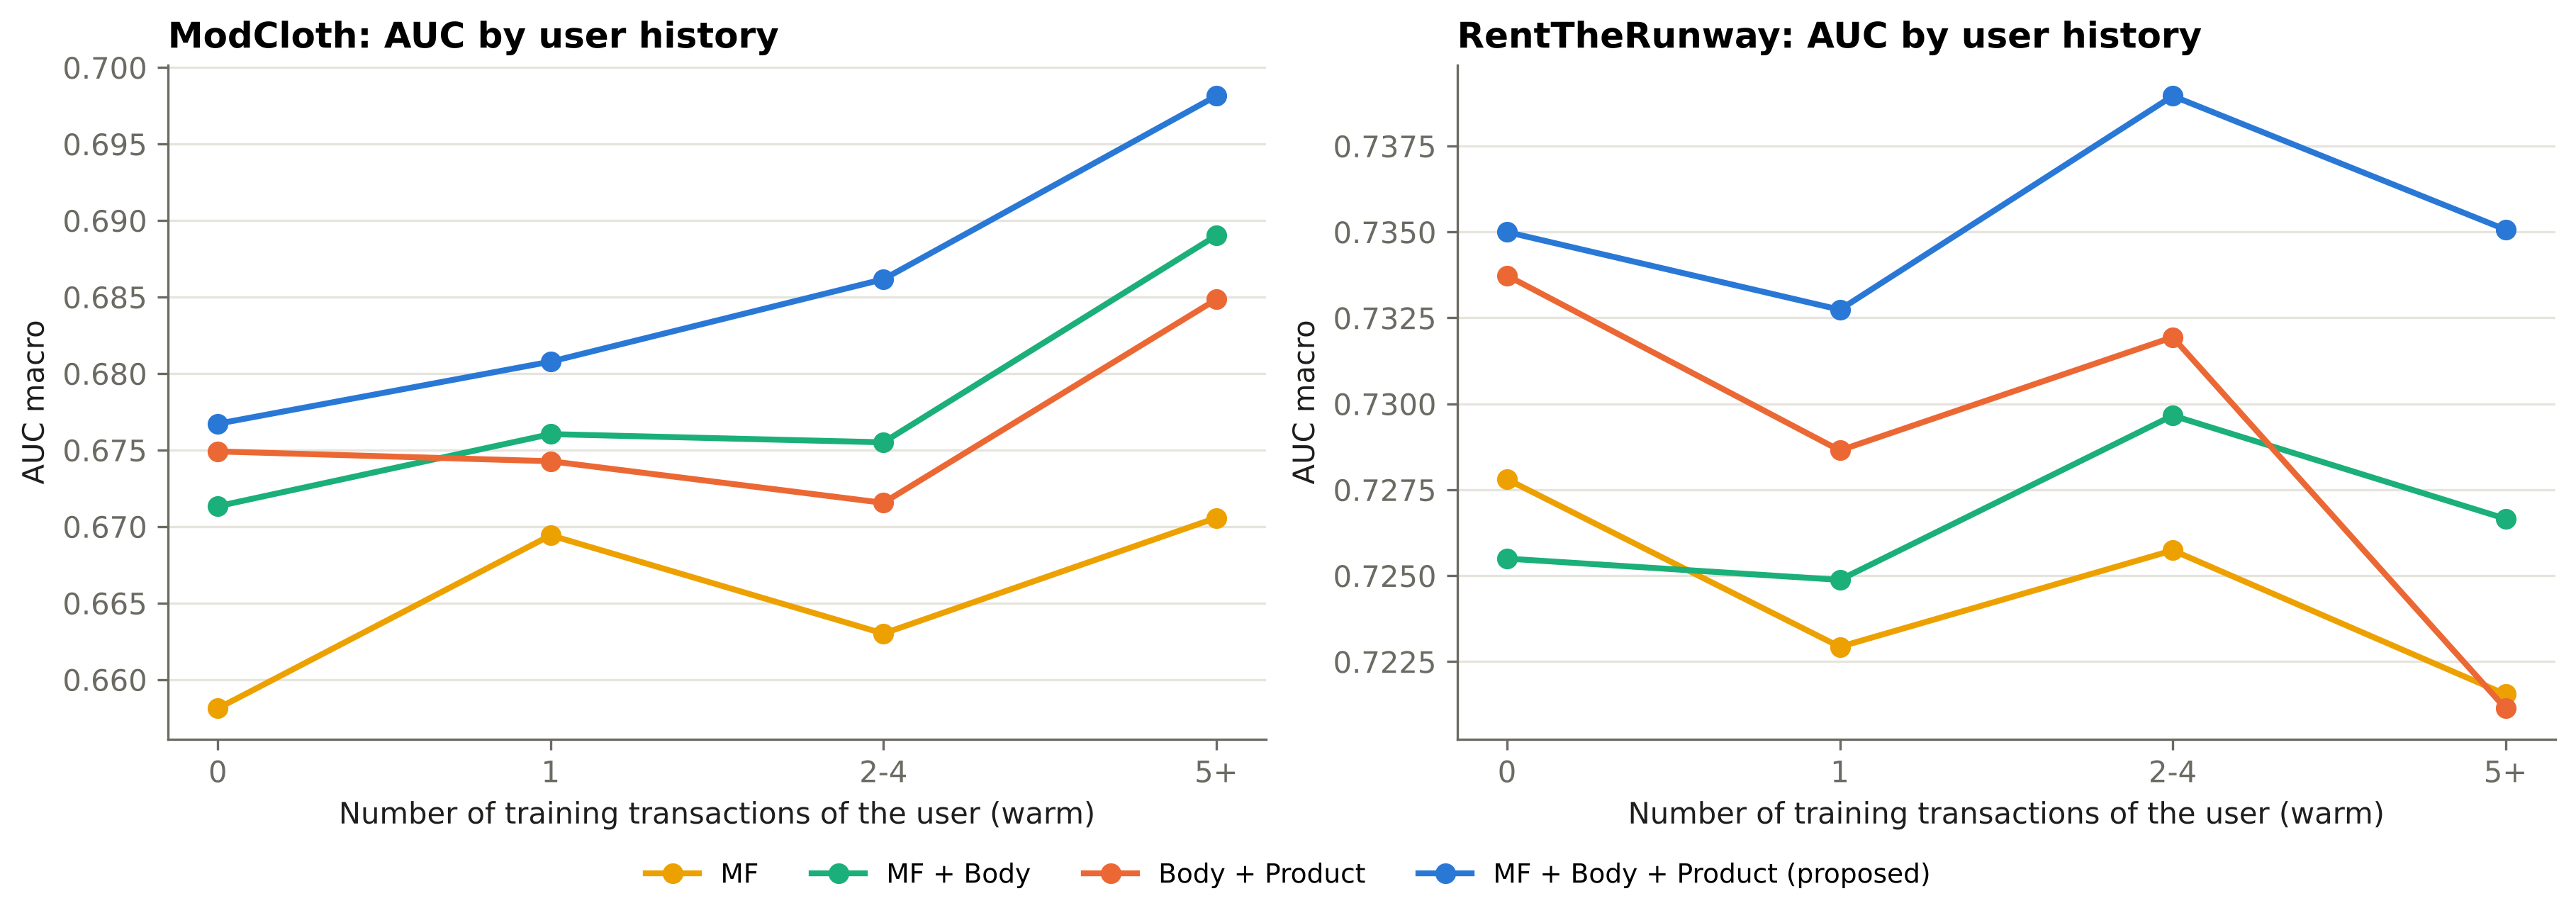
\includegraphics[width=0.85\textwidth]{fig3_auc_by_history.png}
\caption{AUC by number of past transactions of the user (warm protocol)}\label{fig:hist}
\end{figure}

Once users have history, the gap between the proposed model and \texttt{body\_product} widens: +0.015 on ModCloth and +0.007 on RTR for users with 2--4 transactions, and +0.013 and +0.014 for users with 5 or more. The collaborative factor $p_u$ therefore captures personal preferences that measurements do not express. For users with no history the proposed model is still the best, so adding the collaborative part does not hurt new users. This is exactly the desired behaviour of a hybrid: \emph{rely on the body when there is no history, and exploit history when it exists}.

\subsection{Stability across repetitions}
Figure~\ref{fig:box} shows test AUC over the ten repetitions for the five strongest configurations (\texttt{majority} and \texttt{body\_lr} are omitted to keep the scale readable); each point is one repetition with its own data split. The ranking is stable: the proposed model lies to the right of plain MF and MF with body features in every panel and, under the warm protocol, also clearly separates from \texttt{body\_product}; under cold-start the two overlap, matching Table~\ref{tab:cold}. The spread between repetitions (about 0.003--0.007 AUC) is of the same order as the gaps between the strongest models, which is why ten repetitions and paired tests are needed.

\begin{figure}[h]
\centering
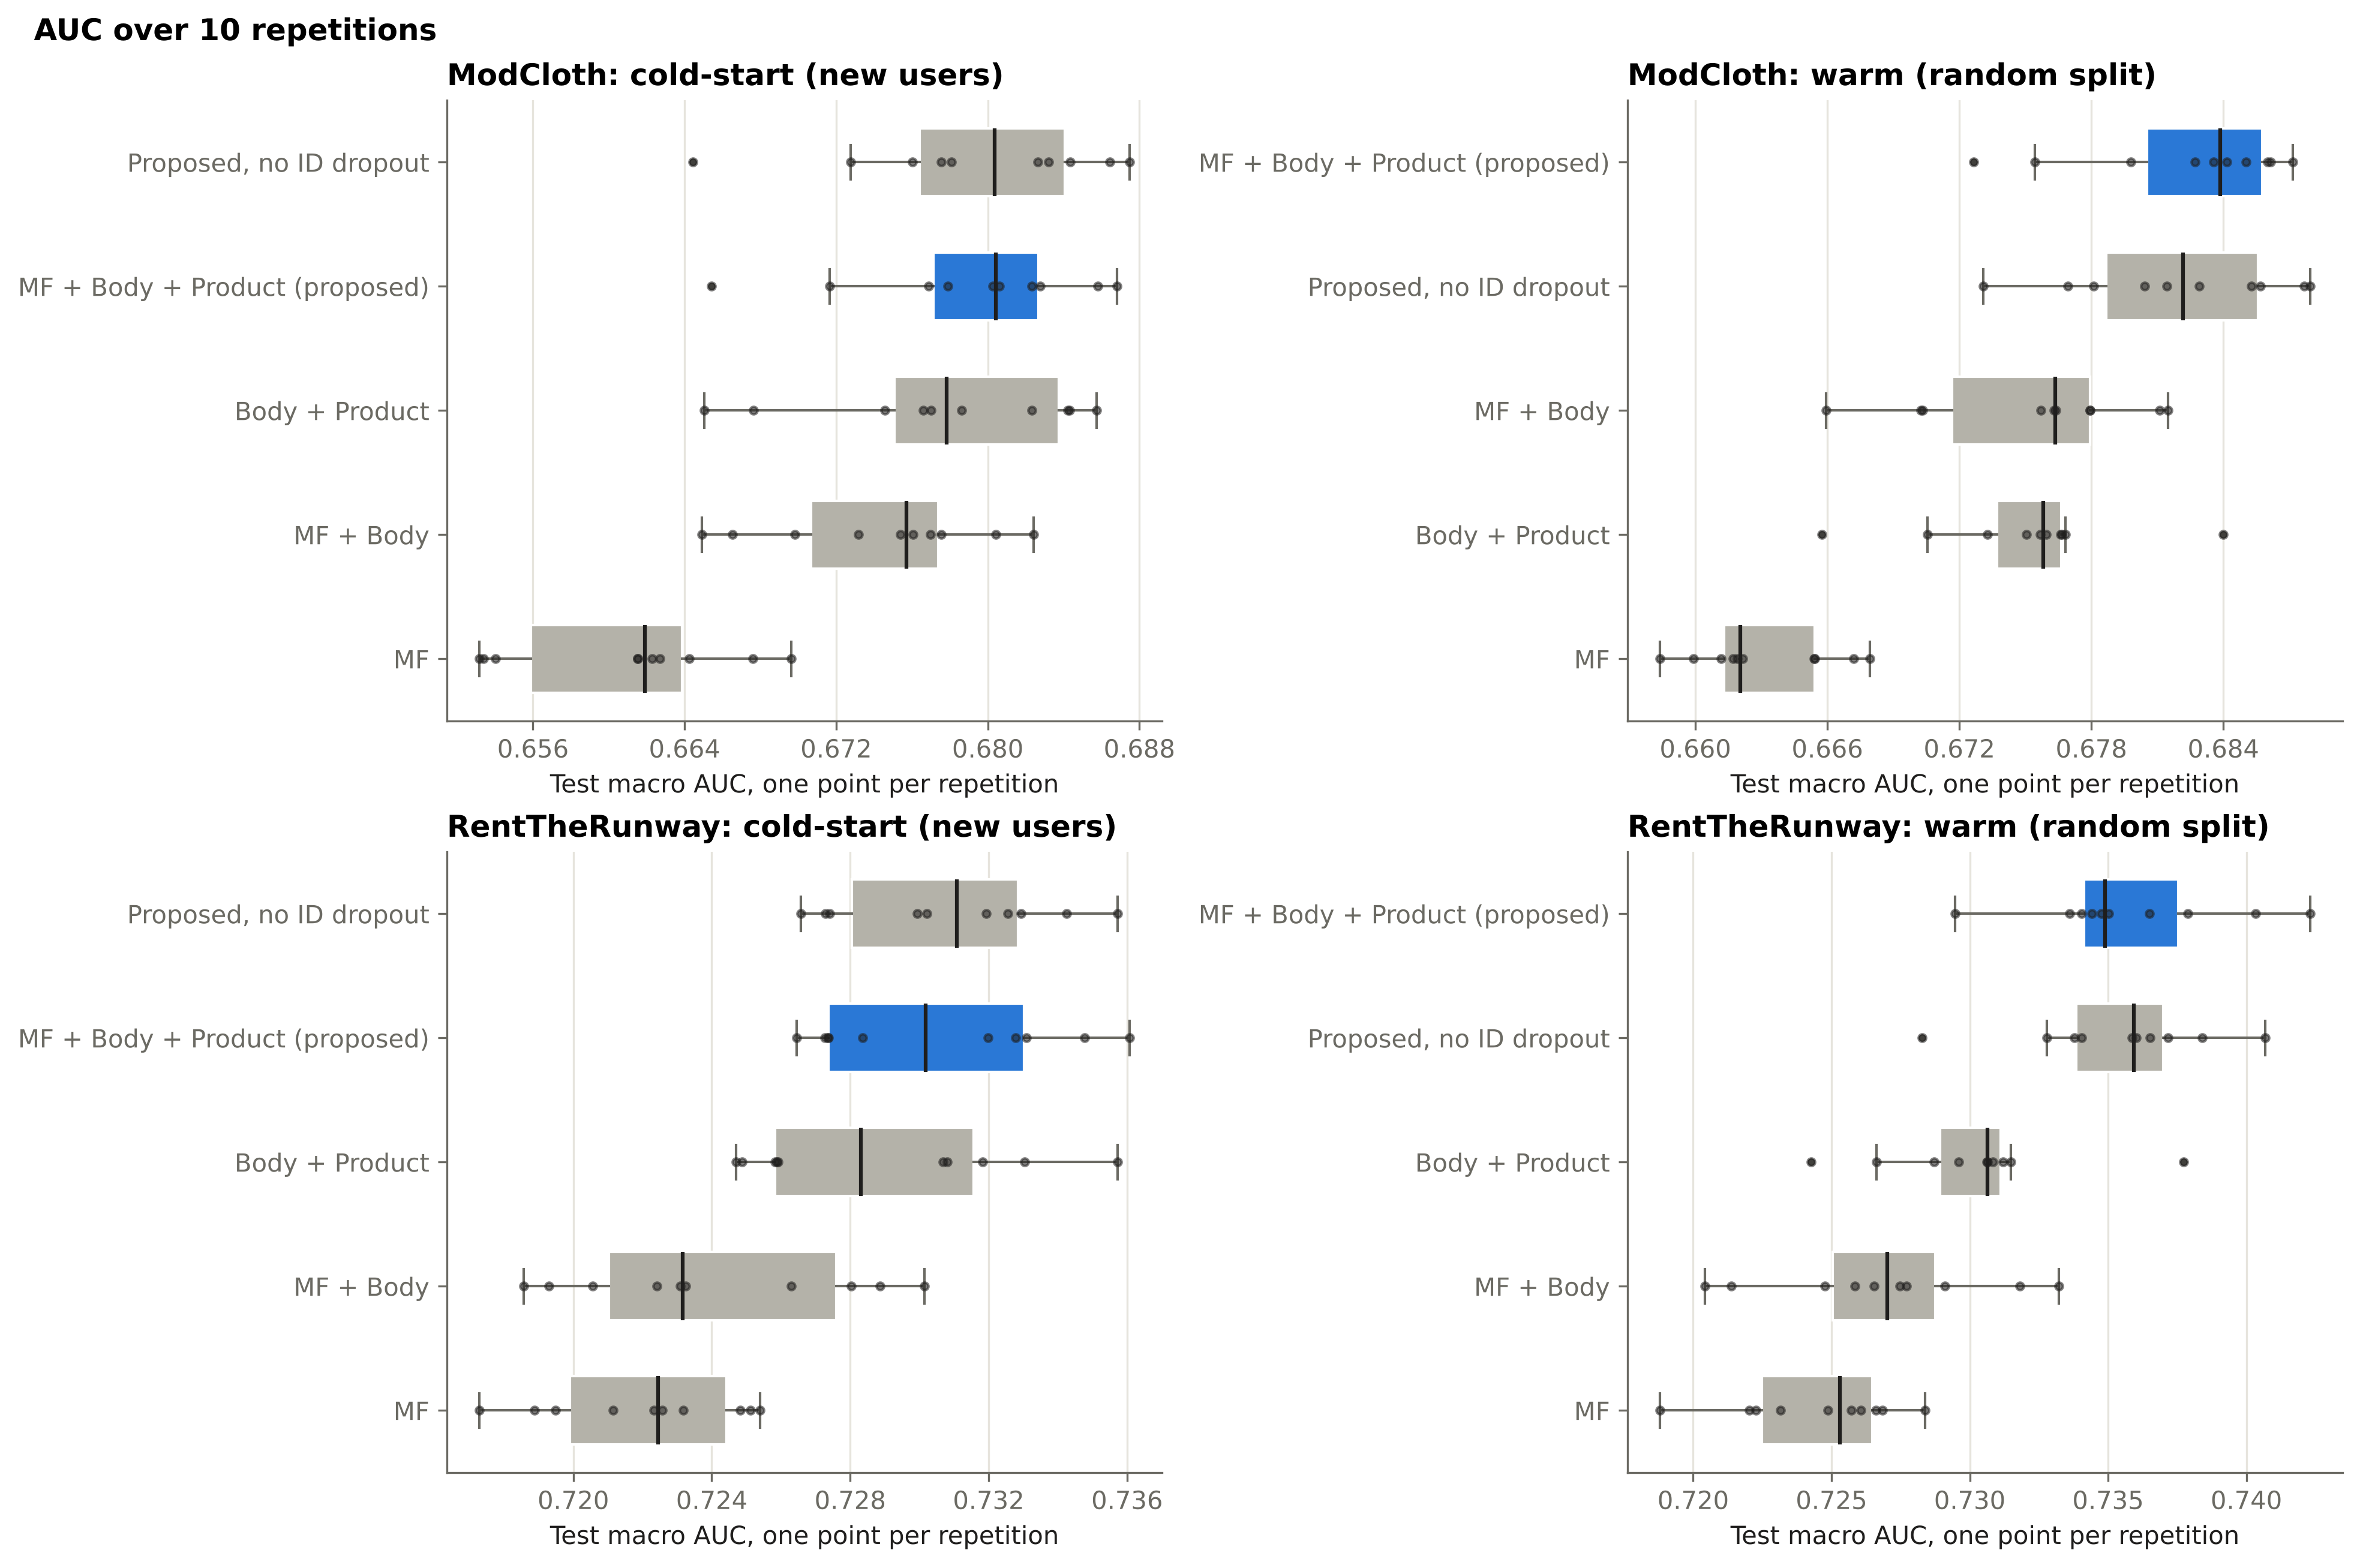
\includegraphics[width=0.9\textwidth]{fig6_auc_boxplot.png}
\caption{Boxplots of test AUC over ten repetitions (seeds 1--10) per model, dataset and protocol; the proposed model is shown in blue}\label{fig:box}
\end{figure}

\subsection{Statistical significance}
Table~\ref{tab:sig} reports $\Delta$AUC of the proposed model against the other models, with 95\% confidence intervals from the paired bootstrap.

\begin{table}[h]
\caption{$\Delta$AUC of the proposed model on the full test set}\label{tab:sig}
\begin{tabular*}{\textwidth}{@{\extracolsep\fill}llcccc}
\toprule
Data & vs. & Protocol & $\Delta$AUC & 95\% CI & $p$ (bootstrap / t-test) \\
\midrule
MC & \texttt{mf} & cold & +0.018 & [0.016, 0.020] & $<$0.01 / $<$0.001 \\
MC & \texttt{mf\_body} & cold & +0.005 & [0.003, 0.006] & $<$0.01 / 0.002 \\
MC & \texttt{body\_product} & cold & +0.001 & [$-$0.000, 0.003] & 0.08 / 0.237 \\
MC & \texttt{mf} & warm & +0.019 & [0.017, 0.022] & $<$0.01 / $<$0.001 \\
MC & \texttt{mf\_body} & warm & +0.007 & [0.005, 0.008] & $<$0.01 / $<$0.001 \\
MC & \texttt{body\_product} & warm & +0.007 & [0.005, 0.009] & $<$0.01 / $<$0.001 \\
\midrule
RTR & \texttt{mf} & cold & +0.009 & [0.007, 0.010] & $<$0.01 / $<$0.001 \\
RTR & \texttt{mf\_body} & cold & +0.006 & [0.005, 0.008] & $<$0.01 / $<$0.001 \\
RTR & \texttt{body\_product} & cold & +0.002 & [0.001, 0.003] & $<$0.01 / 0.002 \\
RTR & \texttt{mf} & warm & +0.011 & [0.010, 0.013] & $<$0.01 / $<$0.001 \\
RTR & \texttt{mf\_body} & warm & +0.009 & [0.008, 0.010] & $<$0.01 / $<$0.001 \\
RTR & \texttt{body\_product} & warm & +0.006 & [0.005, 0.007] & $<$0.01 / $<$0.001 \\
\botrule
\end{tabular*}
\end{table}

The proposed model is significantly better than \texttt{mf}, \texttt{mf\_body} and \texttt{body\_lr} on both datasets and both protocols. Against \texttt{body\_product} the difference is significant under the warm protocol on both datasets (both tests $p < 0.001$) and under cold-start on RTR, but not under cold-start on ModCloth ($p = 0.08$ bootstrap, $0.24$ t-test), consistent with the analysis above: without history the two models share the same form. Removing ID dropout does not change the results significantly ($p > 0.28$): the mechanism does no harm, but gives no clear benefit on these two datasets.

\subsection{Size recommendation}
Table~\ref{tab:sizerec} compares three ways of recommending a size: the best-selling size of the article (what many shops do today), body measurements only, and body measurements combined with purchase history (hybrid).

\begin{table}[h]
\caption{Size recommendation accuracy on \emph{fit} test transactions (warm, mean $\pm$ std over 10 seeds)}\label{tab:sizerec}
\begin{tabular*}{\textwidth}{@{\extracolsep\fill}lcccc}
\toprule
 & \multicolumn{2}{c}{ModCloth} & \multicolumn{2}{c}{RentTheRunway} \\
\cmidrule{2-3}\cmidrule{4-5}
Method & Exact & Within 1 & Exact & Within 1 \\
\midrule
Best-selling size & 25.5 $\pm$ 0.6 & 62.4 $\pm$ 0.6 & 20.9 $\pm$ 0.4 & 51.5 $\pm$ 0.3 \\
Body measurements only & 44.0 $\pm$ 0.7 & 87.7 $\pm$ 0.3 & 39.7 $\pm$ 0.4 & 79.0 $\pm$ 0.3 \\
\textbf{Body + history (hybrid)} & \textbf{51.0 $\pm$ 0.5} & \textbf{91.7 $\pm$ 0.3} & \textbf{44.5 $\pm$ 0.5} & \textbf{82.3 $\pm$ 0.3} \\
\botrule
\end{tabular*}
\end{table}

Body measurements alone almost double the exact-match rate of the best-selling size (25.5\% $\rightarrow$ 44.0\% on ModCloth, 20.9\% $\rightarrow$ 39.7\% on RTR). Adding purchase history adds a further 7.0 points on ModCloth and 4.8 points on RTR. Under cold-start the hybrid and body-only methods coincide because $n_u = 0$ (44.0\% and 40.1\%). Within one size step, the hybrid method reaches 92\% and 82\%, so the recommended size is almost always the size the customer wore or an adjacent one.

\subsection{Discussion}
\paragraph{Comparison with prior work.} Under the warm protocol, which is closest to the random splits of~\cite{misra2018fit,sheikh2019sfnet}, the proposed model reaches 0.682 AUC on ModCloth and 0.736 on RTR. This is above K-LF-ML (0.657 and 0.719) and slightly below SFNet (0.689 and 0.749). The figures are not strictly comparable because pre-processing and splits differ. The proposed model is, however, much smaller, every component has a clear meaning, and it is designed and evaluated specifically for new users, which the earlier works did not do.

\paragraph{Why size selection is separated.} When the fit model was used directly to rank all sizes for one person, very distant sizes (e.g.\ size 28 for a petite customer) sometimes received a $P(\text{fit})$ no lower than the correct size, because the data contain almost no customers wearing sizes far from their body. Separating size selection into a monotone model avoids this failure, while the fit model is used where it is reliable: assessing risk at sizes close to the body.

\paragraph{Business implications.} An online fashion store can deploy the system on the product page: the customer enters a few basic measurements (height, weight, bra size), receives a size together with the risk of a tight or loose fit, and returning customers get increasingly personalised suggestions from their history. Raising the share of correct sizes from about 21--26\% to about 45--51\% is a strong signal for reducing size-related returns; the actual reduction should be measured with an A/B test.

% ====================================================================== SYSTEM
\section{The \texttt{sizerec} System}\label{sec7}

The method is implemented in Python (PyTorch, pandas, scikit-learn) and packaged as the command-line tool \texttt{sizerec}, organised into modules for data handling (\texttt{data.py}), the model and baselines (\texttt{model.py}), training (\texttt{trainer.py}), multi-seed experiments and significance tests (\texttt{experiment.py}), monotone size selection (\texttt{sizing.py}), recommendation with risk and explanations (\texttt{recommend.py}), and the command-line and interactive interfaces (\texttt{cli.py}, \texttt{interactive.py}).

The commands are \texttt{data} (dataset statistics), \texttt{experiment} (experiments and tests), \texttt{train}, \texttt{inspect} and \texttt{recommend}, which can explain its output (\texttt{--explain}) or emit JSON (\texttt{--json}) for integration with other systems. Without arguments, \texttt{sizerec} opens an interactive menu.

\paragraph{Example.} A new customer aged 22, 165\,cm and 57\,kg, bra size 34b, petite, looks at a dress on RTR:
\begin{verbatim}
sizerec recommend models/rtr.pt --item 126335 --height 165cm \
    --weight 57kg --bust-size 34b --body-type petite \
    --age 22 --explain
\end{verbatim}
The base size estimated from the measurements is about 6.2. The system adds 0.3 for the dress category and 0.6 because, according to earlier customers, this article runs small, giving a target of about 7.1, so the closest available size is \textbf{8}. The hybrid model estimates fit 47\%, loose 30\% and tight 23\% at size 8. The loose risk is somewhat high, but the next smaller size (4) has a lower probability of fitting (41\%), so the system keeps size 8. The explanation decomposes the score $t$ into the item--size bias, the collaborative history (zero for a new customer), the body measurements and the size gap, so that the merchant can see why the recommendation was made. For a returning customer with 386 transactions, the weight of the history in the target size is $386/388 \approx 1$ and the collaborative term is non-zero, so the recommendation reflects that customer's own sizing habits.

All experiments can be reproduced with a single script (\texttt{run\_all.sh} or \texttt{run\_all.bat}) with fixed seeds. It computes dataset statistics, runs the pipeline test and the full experiments (7 models, 2 protocols, 10 seeds, significance tests), trains the final models and regenerates every figure, log and the summary spreadsheet in the \texttt{results} folder of the repository.

% ====================================================================== CONCLUSION
\section{Conclusion}\label{sec8}

We built and evaluated a hybrid ordinal matrix factorization model that integrates self-reported body measurements directly into the user representation of MF, for fit prediction and size recommendation in fashion e-commerce. Experiments on ModCloth and RentTheRunway with ten repetitions and significance testing show that:
\begin{enumerate}
\item body measurements mitigate cold-start: on new users the proposed model significantly outperforms plain MF and MF with body features, with AUC 0.679 $\pm$ 0.007 and 0.731 $\pm$ 0.004;
\item the collaborative component pays off once customers have history: for users with two or more purchases the proposed model beats the body-and-product model by up to 0.015 AUC, so the hybrid combines the strengths of both sources;
\item the monotone size-selection procedure raises the exact-size rate from about 21--26\% to about 45--51\%, with more than 82\% of recommendations within one size, which supports the expectation of fewer size-related returns;
\item the whole pipeline is packaged as a reproducible and explainable tool, \texttt{sizerec}.
\end{enumerate}

\paragraph{Limitations.} The public datasets contain no return labels, so the reduction of the return rate is not measured directly. On completely new users the gain over the model without user factors is small, because measurements and product features carry most of the signal. The data are observational and subject to selection bias; we mitigate this by separating size selection but do not apply full causal inference. Self-reported measurements can be inaccurate, and on ModCloth waist and bust are missing in over 85\% of records. Absolute AUC on warm data is still slightly below SFNet.

\paragraph{Future work.} Promising directions are: using review text as a training signal (not as an input at recommendation time)~\cite{baier2019reviews,chatterjee2022reviews}; correcting selection bias with inverse propensity weighting; A/B testing on a live store to measure returns and conversion directly; and adapting the system to the Vietnamese market with brand-specific size charts and body measurements of Vietnamese customers.
